\section{XYZ CNN}



Our model is based on dynamic graph CNN ~\citep{wang2018dynamic}. In this section we explain the architecture of our model and the rationale behind the input we choose for the model.
\subsection{Model}
Figure~\ref{fig:model1} shows our CNN model. The model consists of two parts; features extraction and CNN model. The features extraction tries to pick the appropriate features to learn from. The CNN model is very similar to that used in PointNet architecture in terms of the number of layers and the hyper parameters values. Later, we will explain the changes we have done to the model to speed up the training while maintain the same accuracy. 
\subsection{Feature Extraction} 
We distinguish between two type of features; global and local. Global features are the features associated with the point itself regardless to points neighbors to it. Examples include the point coordinates or point normal (vector with source at the point, perpendicular to the underlying surface and pointing outwards. See Figure~\ref{fig:norm}). Local features associate the point with its neighbors. Example include the distance between the point and its $K$ nearest neighbor points. Our hypotheses  is that learning both the global and local features is essential in order to achieve better accuracy. 



\emph{EdgeFeatures} in Figure~\ref{fig:model1} represent the input to the CNN model such that both global and local information   are well extracted from the input point cloud. For local features, we collect the $K$ nearest points for each point where $K$ is a hyper parameter. We define the function that extract the features of point $i$ as $h(x_{i}, x_{i}-x_{j}), \forall j \in N(i)$ where $x_{i}$ is the coordinates of the point $i$ and $N(i)$ is the local neighborhood of $i$ (the $K$ nearest points)~\citep{wang2018dynamic}. The function basically concatenates the coordinates of the point along with the difference between the point and each of its $K$ nearest neighbors. In that way, a point will have $6\times K$ features; $(x,y,z)$ coordinates of the point concatenated with the difference in each dimension with the coordinates of the $K$ nearest point (Figure~\ref{fig:features}). We apply this feature extraction layer four time, each with different value of $K$. That way we are able to extract a hierarchy of local features that could aide the learning process to achieve faster training. 
\begin{figure}[!tbh]
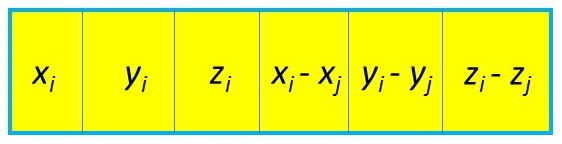
\includegraphics[width=0.5\textwidth]{fig/features.JPG}
\caption{Features per point per point cloud. This tuple is repeated for each point $K$ times for $K$ nearest point where each nearest point give different $(x_{j}, y_{j}, z_{j})$ to compute the difference with. }
\label{fig:features}
\end{figure}

The function as described above is able to extract the proximity in distance between a point and each of the points in its local neighborhood. We can easily recognize that this feature alone can not be very reliable. Figure~\ref{fig:norm} shows example of two pair of points belongs to two difference shapes. Even though the distance is similar, the normal associated with each point is different which can be used as indication that each pair has different underlying surface. For that, we use (in addition to the distance) the point normal during the feature extraction. We apply similar function as this applied for distance but here instead of using the difference, we used the dot product which gives the sense of how much two vectors are similar. Note that the dot product between two vectors returns a single value. Thus, a single point will have $4\times K$ features.

\begin{figure}[!tbh]
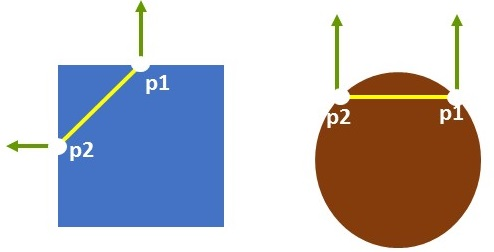
\includegraphics[width=0.4\textwidth]{fig/norm.JPG}
\caption{Distance metric alone between two points of different shapes could be misleading. Aided with point normal, extra features like curvature and shape corners could be learned.}
\label{fig:norm}
\end{figure}

\subsection{CNN Model:}
After extracting the right features, we input each feature layer into a convolutional layer. The output channel in each layer is a hyper parameter that we changed for different experiments. After that we concatenate the output of all convolutional layers into one aggregation layer. The output then goes to three fully connected layers between each there is a dropout layers. The final fully connected layer is the classification layer with 40 classes since the data set we are using (ModelNet40) contains 40 classes 

\subsection{Implementation:}
Here we explain more details about our implementation using TensorFlow. For each input model, we pick (uniformly random) 1024 points from it to train an entire epoch. For each epoch we (uniformly random) pick different set of points. That way we can tackle the irregularity  of the data set and capture different parts of the point cloud and the number of epochs increase. 

Hyper parameters shown in Table~\ref{tab:para} are fixed in all our experiments. We used batch normalization to help train faster and also help as a regularizer. After training an epoch, we run an evaluation to compute the test (out-of-sample) accuracy. We report the maximum accuracy obtained i.e., early stopping. 


\begin{table}[!tbh]
  \caption{Our model fixed hyper parameters.}
  \label{tab:para}
  \begin{tabular}{ccl}
    \toprule
    Parameter &Value & Comments\\
    \midrule
     \# Points & 1024 &  \\
     Batch Size & 32 &  \\
     Max epoch & 300 &  \\
     Learning rate &0.001  &  \\
     Momentum & 0.9 & for batch normalization  \\
     Optimizer & Adam &  \\
     Step Decay & 200000 & for learning rate  \\
     Decay Rate & 0.7 &  for learning rate \\           
     Step Decay & 200000 & for momentum  \\
     Decay Rate & 0.5 &   for momentum  \\     
  \bottomrule
\end{tabular}
\end{table}



